\documentclass[conference]{IEEEtran}
\IEEEoverridecommandlockouts
% The preceding line is only needed to identify funding in the first footnote. If that is unneeded, please comment it out.
\usepackage{cite}
\usepackage{amsmath,amssymb,amsfonts}
\usepackage{float}
\usepackage{algorithmic}
\usepackage{graphicx}
\usepackage{textcomp}
\usepackage{xcolor}
\usepackage{listings}
\usepackage{enumitem}
\usepackage{commath}
\usepackage{color}
\usepackage{hyperref}
\usepackage{siunitx}
\hypersetup{
    colorlinks=true,
    linkcolor=blue,
    filecolor=magenta,      
    urlcolor=cyan,
    pdftitle={Overleaf Example},
    pdfpagemode=FullScreen,
    }
\renewcommand{\tablename}{Tabla}



\definecolor{mygreen}{rgb}{0,0.8,0}
\definecolor{mygray}{rgb}{0.5,0.5,0.2}
\definecolor{mygraycom}{rgb}{0.5,0.5,0.4}
\definecolor{mymauve}{rgb}{0.58,0,0.82}
\definecolor{mygray2}{gray}{.99}

\lstset{ 
	backgroundcolor=\color{mygray2},  
	basicstyle=\footnotesize,      
	breakatwhitespace=false,         % sets if automatic breaks should only happen at whitespace
	breaklines=true,                 % sets automatic line breaking
	captionpos=b,                    % sets the caption-position to bottom
	commentstyle=\color{mygraycom},    % comment style
	deletekeywords={...},            % if you want to delete keywords from the given language
	escapeinside={\%*}{*)},          % if you want to add LaTeX within your code
	extendedchars=true,              % lets you use non-ASCII characters; for 8-bits encodings only, does not work with UTF-8
	firstnumber=1000,                % start line enumeration with line 1000
	frame=single,	                   % adds a frame around the code
	keepspaces=true,                 % keeps spaces in text, useful for keeping indentation of code (possibly needs columns=flexible)
	keywordstyle=\color{blue},       % keyword style
	language=matlab,                 % the language of the code
	morekeywords={*,...},            % if you want to add more keywords to the set
	numbers=none,                    % where to put the line-numbers; possible values are (none, left, right)
	numbersep=5pt,                   % how far the line-numbers are from the code
	numberstyle=\tiny\color{mygray}, % the style that is used for the line-numbers
	rulecolor=\color{black},         % if not set, the frame-color may be changed on line-breaks within not-black text (e.g. comments (green here))
	showspaces=false,                % show spaces everywhere adding particular underscores; it overrides 'showstringspaces'
	showstringspaces=false,          % underline spaces within strings only
	showtabs=false,                  % show tabs within strings adding particular underscores
	stepnumber=2,                    % the step between two line-numbers. If it's 1, each line will be numbered
	stringstyle=\color{mymauve},     % string literal style
	tabsize=2,	                   % sets default tabsize to 2 spaces
	title=\lstname                   % show the filename of files included with \lstinputlisting; also try caption instead of title
}
\renewcommand{\lstlistingname}{Reporte}


\def\BibTeX{{\rm B\kern-.05em{\sc i\kern-.025em b}\kern-.08em
    T\kern-.1667em\lower.7ex\hbox{E}\kern-.125emX}}
    
    
%definicion de excepciones 

\hyphenation{rea-lizan}

\hyphenation{envia-do}

\hyphenation{opti-miza}
%
\hyphenation{extre-madamente}
\begin{document}

\title{Tarea 4 IPD-432\\
{%\footnotesize \textsuperscript{*}Note: Sub-titles are not captured in Xplore and
}
%\thanks{Identify applicable funding agency here. If none, delete this.}
}

\author{\IEEEauthorblockN{ Reinier López Ahuar}
	\IEEEauthorblockA{\textit{ Departamento de Electrónica} \\
		\textit{Universidad Técnica Federíco Santa María}\\
		Chile, Valparaíso \\
		reinier.lopez@sansano.usm.cl}
\and
\IEEEauthorblockN{José Cayo Torrejón }
\IEEEauthorblockA{\textit{Departamento de Electrónica} \\
\textit{Universidad Técnica Federico Santa María}\\
Chile, Valparaíso \\
jose.cayo.14@sansano.usm.cl}
}
\maketitle
% \begin{abstract}
% \end{abstract}
% \begin{IEEEkeywords}
% component, formatting, style, styling, insert
% \end{IEEEkeywords}
% \section{Introduction}
% This document is a model and instructions for \LaTeX.
% Please observe the conference page limits. 
\section{Introducción}
En este informe se presenta  la metodología empleada para implementar un \textit{device} con la misma funcionalidad requerida en la Tarea 3, la cual consiste en realizar ciertas operaciones a dos vectores, provenientes de comunicación serial en la NEXYS4 DDR. Además, se emplea la herramienta Vitis HLS 2021.1 para el diseño de hardware  en el cálculo  de la distancia euclidiana. Además, con este objetivo se utilizan las herramientas de Vivado y Vitis y la implementación en la Zybo.  La decisión de diseño repercute directamente  en las medidas fundamentales de la implementación de un sistema digital conocidas como latencia y \textit{throughput}. La latencia se puede definir como el número de ciclos de reloj necesario en un sistema para generar una salida dada una entrada determinada, mientras que el \textit{throughput} es la cantidad de salidas  por unidad de tiempo.   A continuación, se resume el diseño del procesador de vectores usando HLS para Nexys4 DDR y el empleo de un sistema heterogéneo en SoC Zynq, y se muestran  las principales observaciones.\par
  %A continuación se resumen las principales características de un FPGA. 
  \section{Procesador de vectores usando HLS para Nexys4 DDR} 
 
\subsection{Vitis HLS}

\subsubsection{Código de alto nivel}
Para la implementación del bloque del cálculo de la distancia  euclidiana, se establece la creación de una función que utilice la misma arquitectura de las demás operaciones. Esta función posee las siguientes entradas:

\begin{itemize}
    \item A[M] y B[M]: Los vectores de entrada a los cuales se realiza el cálculo de la distancia Euclidiana, cada uno de M elementos de longitud.
    \item C: La dirección que contiene el resultado de la distancia Euclidiana.
\end{itemize}

Cabe destacar que al usar punteros, no se requiere establecer un valor de retorno. Además, dichas entradas se encuentran ligadas a un tipo de variable gracias al uso de la palabra reservada \textit{typedef}. Estas definiciones corresponden a T y T2 para el  resultado C y para los vectores A[M] y B[M], respectivamente.

Los valores de entrada se procesan mediante un ciclo \textit{for}, en donde se calcula la diferencia elemento a elemento, las cuales se agregan a una variable que contiene la sumatoria. Finalmente se utiliza la función \textit{sqrt}, proveniente de la librería \textit{math.h}, al valor de dicha sumatoria y se entrega al puntero de resultado.

\subsubsection{Pragmas utilizados}
Los pragmas se utilizan para que el bloque IP siga la arquitectura del \textit{Processing Core} de interés, así como obtener una implementación que no sobrepase los recursos disponibles de la FPGA Nexys4. Los pragmas utilizados en la implementación son los siguientes:
\begin{itemize}
    \item ARRAY PARTITION: Permite realizar particiones vectores en secciones más pequeñas. El desarrollo de la tarea 3 considera una memoria de tipo SIPO (\textit{Singular input Parallel Output}), por lo que, al querer evitar realizar cambios en la arquitectura se decide particionar los 2 vectores de forma completa, y así lograr una implementación idéntica.
    \item PIPELINE: Permite segmentar las operaciones realizadas en el código de alto nivel. Se utiliza  para lograr una implementación con la menor cantidad de recursos posible, a cambio de una mayor latencia. Además, se utilizan los parámetros por defecto.
\end{itemize}

Se realizan pruebas preliminares con el pragma UNROLL, que reduce la cantidad de comparaciones, y en contraste, una mejora considerable en la latencia. No obstante, la FPGA a usar no posee los recursos necesarios para implementar dicha estrategia, llegando a estimar el uso de 500 DSP, por lo que al quererla implementar en la tarjeta se deben utilizar LUTs en su lugar, agotando los recursos (en dicho caso, la implementación en Vivado utilizaba más de 70000 LUTs, mientras la tarjeta solo tiene disponible 66000). 


\subsubsection{Estimación de rendimiento y recursos}
Una vez completado el proceso de síntesis, el programa entrega un estimado del rendimiento y el uso de recursos, dado por la tabla \ref{tab:Resource_estimate1}. En ella se encuentra tanto el estimado del módulo en su totalidad como el bucle presente en el código, considerando un reloj de 100 MHz (período de 10 ns). Es posible apreciar que los pragmas permiten obtener una implementación con uso tentativamente óptimo de recursos. No obstante, cabe destacar que el uso de recursos considera solamente la instancia del bloque por si solo, por lo que existe la posibilidad que incremente los recursos que el bloque requiera para implementarse en la FPGA, en especial en el uso de LUTs.

Con respecto a los valores de latencia presentes en la tabla \ref{tab:Resource_estimate1}, se determina que la implementación por HLS posee una mejor latencia que implementaciones anteriores. Para el caso de la tarea 2 (última implementación), el cálculo de la distancia Euclidiana presenta una latencia de más de 5000 ciclos. Dado que es una estimación, se debe medir la latencia con un analizador lógico, sea interno o externo.

\begin{table}[!ht]
\caption{Estimación y rendimiento del bloque Euclidiano, al ser sintetizado en Vitis HLS}
\label{tab:Resource_estimate1}
\begin{tabular}{|l|l|l|l|l|l|}
\hline
Módulo/loop & Latencia (Ciclos) & Latencia(ns) & DSP & FF & LUT \\ \hline
EucHW & 1093 & 10930 & 3 & 569 & 6965 \\ \hline
loop & 1027 & 10270 & - & - & - \\ \hline
\end{tabular}
\end{table}

\subsubsection{Estructura Bloque IP Generado}
Una vez exportado el código HLS, se obtiene un bloque IP presente en la figura \ref{fig:HLS_block1}. En ella se aprecian las siguientes entradas y salidas.

\begin{itemize}
    \item A\_n: El Elemento n-ésimo del vector A. Dentro de la implementación final, se encuentran 1024 conexiones asociadas. Cada elemento tiene el tamaño de un caracter (8 bits).
    \item B\_n: Análogo al caso A\_n.
    \item ap\_clk: Entrada en donde ingresa la señal de reloj del Processing Core
    \item ap\_rst: Señal de reseteo. No es utilizada, por lo que se deja dicha entrada siempre en 0.
    \item ap\_start: Entrada en donde se ingresa una señal de disparo para empezar con el cálculo de la distancia Euclidiana
    \item ap\_done: Salida que entrega una señal de disparo una vez terminado el cálculo de la distancia euclidiana.
    \item C: Salida que contiene el resultado de la distancia Euclidiana.
\end{itemize}
Se puede apreciar que ciertos nombres de los puertos mantienen los nombres definidos en la función presente en Vitis HLS, gracias al uso de punteros en su definición previa. Existen otros puertos en el Bloque IP que al no requerirse en la arquitectura de la tarea anterior no son usados, quedando la conexión "al aire". 
\begin{figure}
    \centering
    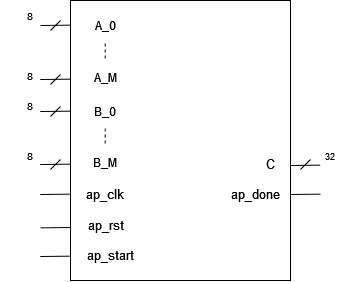
\includegraphics[width=\columnwidth]{Imagenes/Bloque_IP.drawio.png}
    \caption{Bloque IP generado por Vitis HLS, en donde se detallan puertos de entrada y salida}
    \label{fig:HLS_block1}
\end{figure}

\subsection{Versión del dispositivo a usar}
    Como se hace mención anteriormente, se utiliza el \textit{device} diseñado en la tarea 3, la cual sigue el paradigma \textit{full-pipeline}, en donde, para el contexto de dicha tarea, se segmentaba la operación de la distancia de Manhattan, con el fin de lograr un mayor \textit{throughput} en función a un paradigma completamente combinacional. El desarrollo de este \textit{device} permitieron lograr un buen uso de recursos, a cambio de frecuencia de reloj; dicha implementación logra funcionar a una frecuencia de 80 MHz. Considerando que esta implementación presenta una holgura de recursos considerable, se busca integrar el \textit{device} con todas las operaciones, en donde la distancia Euclidiana se lleva a cabo mediante el bloque IP de Vitis HLS.
    
    Una vez implementada el diseño del \textit{device} en la FPGA, los vectores A y B se transmiten desde el ordenador mediante una interfaz de Matlab. Debido a ciertas observaciones, se modifica la manera de seleccionar el puerto serial; para ello se mantiene el método para encontrar la lista de puertos disponibles, pero en vez de siempre usar el primer elemento de dicha lista, se establece una ventana en donde se solicita al usuario seleccionar el puerto serial que utiliza la tarjeta en ese momento. Esto evita problemas si se llega a tener conectado más de 2 dispositivos USB que usen este periférico, en donde la estrategia anterior tiene la posibilidad de entregar el puerto equivocado. Cabe destacar que el usuario es el responsable de conocer el puerto que la FPGA utiliza y, en caso de equivocarse, sólo se debe ejecutar nuevamente el \textit{script}, y posteriormente elegir el puerto correcto.\par
    
    Otro cambio realizado a la interfaz de MATLAB proviene en la conversión de los datos provenientes del cálculo de la distancia de Manhattan. El método utilizado en la tarea 3 se encuentra obsoleta, por lo que se cambia por el método \textit{dec2bin}, en donde se realiza la conversión a binario de los datos obtenidos por UART, considerando la significancia de cada set de 8 bits recibido. Posteriormente se concanetan considerando su respectiva significancia de bits, para luego retransformar el resultado nuevamente a decimal. Existen otros métodos obsoletos que manejan la comunicación UART, que tambien fueron ajustados a una versión más reciente de MATLAB.
    
    La principal modificación considerada en el diseño de la estructura del dispositivo es el almacenamiento de los datos contenidos en los vectores. Lo anterior se llevaba a cabo mediante la instanciación de bloques de memoria (BRAM) a través bloques IP provenientes de la herramienta Vivado. Si bien el empleo de las BRAM reduce significativamente los recursos lógicos utilizados por la tarjeta de desarrollo, una de las características que resulta un inconveniente para acelerar las operaciones en los vectores A y B es el acceso a los datos que estos bloques almacenan. Sólo se tiene acceso  a un elemento de la memoria, dado a que el bloque IP sólo puede usar una sola dirección de memoria como entrada, por lo que sólo se puede acceder un dato por ciclo de reloj, lo cual no es posible aplicar un tipo de paralelismo.\par

    En este diseño, se emplea el uso de \textit{unpacked arrays}, siendo un nuevo tipo de variable disponible en SystemVerilog, el cual permite definir las dimensiones de la misma, similar a otros lenguajes de programación. La definición de los datos como  salida de un módulo  se muestra a continuación:
    \begin{align}
       \text{output}  \ \text{logic}  \ \text{unsigned}  \ [bits-1:0] \ Dato \ [N - 1:0],
    \end{align}
 , donde $[bits-1:0] $ define la cantidad de \textit{bits} en cada elemento del vector, mientras que $[N - 1:0]$ define la cantidad de elementos. Esta descripción permite la implementación de una estructura tipo \textit{Serial-Input Parallel-Output}  (SIPO). Tal como lo menciona su nombre, esta estructura da acceso a los datos que almacena en forma paralela, lo que permite acelerar las operaciones en los vectores mediante ciertas estrategias de parametrización. \par
 Las operaciones a implementar son similares a aquellas presentes en la Tarea 2. Estas operaciones son las siguientes:
\begin{itemize}
    \item readVec, para la lectura de vectores
    \item sumVec, para la suma de vectores, elemento a elemento
    \item avgVec, para el promedio de vectores, elemento a elemento
    \item manDist, para la distancia de Manhattan entre los 2 vectores.
    \item eucDist, para la distancia Euclidiana entre los 2 vectores.
\end{itemize}
 La Figura \ref{fig:Diagrama}  muestra el diagrama de bloques de alto nivel para coprocesador de operaciones sobre vectores. La funcionalidad requerida se detalla a continuación:
        \begin{figure*}[]
    \centering
    \includegraphics[scale=0.45]{Imagenes/Diagrama de bloques.pdf}
    \caption{Diagrama de bloques de alto nivel para el coprocesador para operaciones sobre vectores.}
    \label{fig:Diagrama}
\end{figure*}
\vspace{0.2cm}
 \begin{itemize}
\setlength\itemsep{1em}
    \item Mediante la interfaz UART se envían dos vectores A y B desde el \textit{host} a través de un \textit{script} de Matlab.
    \item Los vectores recibidos se almacenan en los bloques de registros de forma serial a través de los \textit{arrays unpacked } correspondientes a cada vector. 
    \item El bloque \textit{Processing Core} recibe la orden del \textit{host} y realiza distintas operaciones en los vectores almacenados: i) Envía las operaciones mediante la interfaz UART hacia el \textit{host} ii) mediante los puertos de entrada-salida (I/O) muestra la distancia de Manhattan en el display de 7 segmentos.
\end{itemize}

Dentro de la misma Figura \ref{fig:Diagrama}, se aprecia también los módulos a diseñar para el coprocesador, cuya funcionalidades se describen a continuación:
\begin{enumerate}
\setlength\itemsep{1em}
    \item \textit{Clock}: Este módulo se encuentra disponible en el \textit{IP Catalog} de la herramienta Vivado. Permite diseñar un reloj con la frecuencia requerida por el usuario a partir de un reloj conocido. En este diseño la máxima frecuencia de operación es de  30 MHz.
    \item \textit{Uart\_basic}: Se emplea  un módulo diseñado por  Felipe Veas, disponible en el repositorio IPD 432. El diseño implementa un \textit{Universal Asynchronous Receiver/Transmitter} (UART). Permite configurar la frecuencia del reloj a operar y el \textit{baud rate}. Consta además de entradas para habilitar escritura o lectura, así como banderas o bits indicadores para ofrecer información al usuario en el proceso de transmisión o recepción de datos.
    \item \textit{Mux}: Este módulo se implementa con el objetivo de multiplexar las señales hacia los distintos bloques de memoria o hacia el módulo \textit{Command\_Decoder\_Op} para realizar las operaciones requeridas.
    \item  \textit{Command\_Decoder\_Op}: Este módulo, en función de la operación especificada por el usuario, habilita las señales de \textit{trigger} para iniciar la funcionalidad.
    \item \textit{Driver\_RAM}: Tiene la función es escribir cada dato  de 8 bits entregado por el multiplexor en los bancos de registros para los N datos de cada vector. Se instancia un módulo para cada vector. Se aprecia que en este módulo está una de las principales modificaciones del diseño, donde una vez recibidos y almacenados todos los datos en los registros, es posible el acceso a éstos en forma paralela.
    \item \textit{Processing\_core}: En este módulo se ejecutan todas las operaciones indicadas por los \textit{triggers} provenientes del bloque \textit{Command\_Decoder\_Op}. El resultado es enviado posteriormente al módulo \textit{Uart\_basic} y el módulo \textit{UnsignedBcd} si se requiere, en este caso sólo para la distancia de Manhattan. En este módulo está contenido el resto de las modificaciones para obtener la versión de \textit{fully-combinational datapath}. Los datos de los vectores almacenados previamente están disponibles en forma paralela para este módulo.   
    \item \textit{UnsignedBcd}: Se emplea un módulo diseñado por  Felipe Veas. Este módulo es una implementación del algoritmo double-dabble. Su función es convertir un número binario a BCD. 
    \item \textit{Sweep}: Se emplea un módulo diseñado por Ángel Cedeño (angel.cedeno@sansano.usm.cl) para mostrar cada dígito del dato en el display de 7 segmentos, correspondiente a una frecuencia de 1KHz.
    \item \textit{BCD\_to\_sevenSeg}: Permite convertir las señales para que se muestren en el display de 7 segmentos. 
\end{enumerate}

Finalmente, se agregan 2 puertos que permiten sacar las señales de disparo ap\_start y ap\_done fuera de la tarjeta. Se encuentran el los pines 1 y 2, respectivamente, del Pmed Header JA. Esto tiene como finalidad medir la latencia del bloque generado por Vitis HLS.
% \subsection{Operaciones de vectores implementadas}
%  Tal como se menciona anteriormente, las operaciones se realizan dentro del módulo \textit{Processing core} como se muestra en la Figura \ref{fig:Processing_Core2}. 
%  \begin{figure}[]
%     \centering
%         \includegraphics[scale=0.30]{Imagenes/Processing_Core2.pdf}
%     \caption{Diagrama del módulo Processing\_Core2.}
%     \label{fig:Processing_Core2}
% \end{figure}

% Se utilizan máquinas de estado para describir la funcionalidad de cada  operación, con excepción de la operación \textit{manDist}. Al tener acceso a todos los datos, es posible realizar todas las operaciones en un solo estado, a diferencia del diseño original presente en la Tarea 2. En la Figura \ref{fig:tohost_FSM} se aprecia el diagrama de estado responsable de enviar los datos almacenados en los registros hacia el \textit{host}. Los estados de la máquina se describen a continuación:

% \begin{itemize}
%     \item Idle: Estado inactivo de envío, a espera de la operación correspondiente
%     \item Memory: Se recibe la señal \textit{trigger} de la operación, por lo que se procede a la lectura de los datos para su envío. Antes de pasar al estado de transmisión, se espera un número de ciclos dado por INCREMENT\_DELAY\_CONTINUOUS. La mayoría de las operaciones solo requiere 3 ciclos para tener datos válidos (se realizan pruebas con valores menores, pero el diseño no funciona correctamente), aunque eso cambia para la operación de Manhattan en estrategia de \textit{pipeline}, lo cual se explica más adelante.
%     \item Tx: Ya con un dato válido se entrega la información a la interfaz UART para su envío al \textit{host}.
%     \item Busy: Estado que implica que aún no se completa la transmisión del dato anterior. Una vez terminada la transmisión se procede con el siguiente elemento, o se termina de operar en caso de no tener más datos que enviar.
% \end{itemize}
%  \begin{figure}[]
%     \centering
%         \includegraphics[width=\columnwidth]{Imagenes/tohost_v2(1).png}
%     \caption{Diagrama de estado del módulo \textit{To\_Host\_FSM}.}
%     \label{fig:tohost_FSM}
% \end{figure}

% Esta máquina de estado se instancia para cada operación por separado, al ser una estrategia completamente combinacional en donde se multiplexa las salidas correspondientes para manejar la comunicación entre ambos procesadores. Esto se logra gracias a que la definición de esta máquina de estado permite realizar adaptaciones a cada operación, como lo es para el caso de la operación \textit{manDist}, en donde se envía el valor final en secciones de 8 bits mediante la misma estrategia de envío de elemento a elemento.\par

% También se aprecia que, a pesar de tener acceso a todos los datos, la velocidad de la operación se ve limitada al uso del protocolo de transmisión UART, al ser el cuerno de botella de la implementación. El diseño de esta máquina de estados para la operación de readVec, es una modificación de la propuesta en la Tarea 2 con el nombre \textit{To\_Host\_FSM}, que en comparación presenta una menor cantidad de estados y es más moldeable que su contraparte con implementación BRAM.\par

%   La  implementación  de sumVec se realiza de forma paralela mediante un ciclo \textit{for} disponible en SystemVerilog; este \textit{for} difiere de su comportamiento convencional en otros lenguajes, que en vez de realizar operaciones secuenciales, el programa determina el tipo de conexiones de hardware a realizar en base a la condición presente en el \textit{for} mismo.  En comparación con el diseño de la Tarea 2, donde el tiempo de la operación se ve limitado por el acceso de los datos, este diseño permite optimizar el  tiempo requerido. En otras palabras, excluyendo el tiempo requerido para el UART, al ser dependiente del protocolo de comunicación,  cuando se tiene acceso a cada uno de los datos de forma serial,  es necesario N ciclos de reloj para operaciones de suma, donde N es la cantidad de elementos del vector, mientras que en este nuevo diseño, todas las operaciones se realizan de forma paralela, sin requerir una cantidad de ciclos dependiente del número de datos. \par

\subsection{Implementación en Vivado}

\subsubsection{Recursos}
Ya con todos los cambios realizados al \textit{device} en orden, se procede a realizar la implementación total del mismo, obteniendo los resultados presentes en la tabla \ref{tab:IMP_vivado}. Se puede apreciar que la integración de la operación Euclidiana alcanza a convivir con el resto de los módulos del \textit{device} sin agotar los recursos de la tarjeta, logrando afirmar la hipótesis realizada en la tarea 3. 

\begin{table}[!ht]
\centering
\caption{Reporte de recursos lógicos de la Implementación (Place Design) del código fuente del \textit{Processing Core}, incluyendo la distancia Euclidiana}
\label{tab:IMP_vivado}
\begin{tabular}{c|c|c}
\hline
\multicolumn{1}{c|}{Recurso}  & N°&\%Uso  \\ \hline
Slice LUTs    &  53467 & 84.33    \\ \hline
LUT as Logic    & 53411 & 84.24   \\ \hline
LUT as Memory    & 56 & 0.29   \\ \hline
Slice Registers & 30895 & 24.37     \\ \hline
Register as Flip Flop & 30895 & 24.37     \\ \hline
F7 Muxes & 4232 & 13.35       \\ \hline
F8 Muxes           & 2048 & 12.92         \\ \hline
DSP           & 3    & 1.25      \\ \hline

\end{tabular}
\end{table}

No obstante, la tabla anterior no entrega los recursos que ocupa en particular el bloque IP correspondiente a la distancia Euclidiana. Dicha información se encuentra en la tabla \ref{tab:EUC_resource_only}, en donde se aprecia que gran parte de los recursos de LUTs disponibles en la tarjeta son usados en su mayoría por este bloque, y un porcentaje no despreciable de Flip Flops. Si se compara con las estimaciones presentes en la tabla \ref{tab:Resource_estimate1}, la diferencia es considerable, en especial para el caso de los LUTs. Esto se debe a que dicha estimación sólo considera la caja negra del bloque Euclidiano. Al realizar conexiones directas con la memoria SIPO de ambos vectores, el bloque IP requiere mayor recursos para mapear las direcciones, y por tanto, el bloque requiere un mayor número de LUTs. A pesar de esta diferencia, lo que importa es el uso total de recursos, por lo que la hipótesis sigue siendo válida.

\begin{table}[!ht]
    \centering
    \caption{Reporte de recursos utilizados por el bloque IP responsable del cálculo de la distancia Euclidiana}
    \label{tab:EUC_resource_only}
    \begin{tabular}{|l|l|}
    \hline
        Recurso & N° en Uso \\ \hline
        Slice LUTs & 36990 \\ \hline
        Flip Flops & 3978 \\ \hline
        DSP & 3 \\ \hline
    \end{tabular}
\end{table}


\subsubsection{Timing}

Con respecto a los reportes de timing, se logra una implementación funcional con una frecuencia de 70 MHz, lo cual difiere con la frecuencia máxima teórica reportada por Vitis HLS, que es de aproximadamente 140 MHz. Similar a la estimación de recursos, esta diferencia es ya que sólo considera el bloque IP por separado y no el resto de los módulos, el protocolo de comunicación y demás interconexiones. Como respaldo, se adjunta el reporte general de \textit{timing} entregado por Vivado, dado por la tabla \ref{tab:EUC_timing}.

\begin{table}[!ht]
    \centering
    \caption{Reporte de timing para la implementación}
    \label{tab:EUC_timing}
    \begin{tabular}{|l|l|l|}
    \hline
        WNS (Worst Neg. Slack) & TNS (Total Neg. Slack) & WHS (Worst Hold Stack) \\ \hline
        0.129 & 0.0 & 0.009 \\ \hline
    \end{tabular}
\end{table}

\subsubsection{Medición de latencia}

Para medir la latencia se utilizan los 2 pines habilitados para medir la latencia del cálculo de la operación euclidiana. Para ello se toma el tiempo en que ocurre el canto de subida de la señal ap\_start, ligada a la señal \textit{etrigger} del decodificador, y el canto de subida de la señal ap\_done. La medición de dichas señales se realiza mediante el uso del Analizador Lógico presente en el Analog Discovery, ya que posee la suficiente frecuencia de muestreo para medir las señales a la frecuencia máxima obtenida. Se intenta en un principio reducir la frecuencia y probar con el Analizador lógico provisto por el profesor Gonzalo Carvajal, pero, o no funciona de forma correcta la comunicación o, en caso de lograr comunicación, la latencia difiere demasiado con su contraparte estimada.

La medición de la latencia se aprecia en la figura \ref{fig:latency_measure}, en donde se determina que el intervalo de tiempo entre ambos cantos de subida es de aproximadamente 15.61 us. Considerando una frecuencia de reloj de 70 MHz, la cual fue usada en el experimento. La cantidad de ciclos que tarda la distancia Euclidiana en calcularse está dado por:

\begin{equation*}
    Ciclos=\frac{\Delta X}{T_{clk}} =\num{15.61e-6}*\num{70e6}=1092.7
\end{equation*}

Se obtiene que el cálculo tarda alrededor de 1092 ciclos en obtener la distancia euclidiana, lo cual se acerca a lo estimado por la tabla \ref{tab:Resource_estimate1}. Las diferencias se pueden explicar por la frecuencia de muestreo del analizador usado, la cual es de 100 MHZ, estado un tanto alejado de lo recomendado (140 MHZ). Sin embargo, el canto de subida es detectado por el dispositivo teniendo una medición factible, aunque no con la mejor precisión.
\begin{figure}[h]
    \centering
    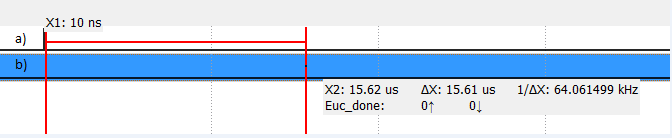
\includegraphics[width=\columnwidth]{Imagenes/Latency_measure_highlight.PNG}
    \caption{Medición de latencia temporal del cálculo de la distancia euclidiana, con frecuencia de reloj a 70 MHz, en función de las señales de disparo a) ap\_start y b) ap\_done. }
    \label{fig:latency_measure}
\end{figure}

  \section{Sistema heterogéneo en SoC Zynq}

 En esta sección se diseña otra  versión del coprocesador. Se considera solamente la implementación de la distancia euclidiana debido a que la lógica programable de la xc7z010-clg400-1 consta de menos recursos disponibles. 
 \subsection{Vitis HLS}
 Los archivos necesarios para obtener el IP desde Vitis tienen el mismo nombre  y estructura que los archivos de código fuente y simulación de  la sección anterior. Las modificaciones fundamentales consisten en 
 \begin{enumerate}
     \item Concatenar los vectores A y B. \label{Concatenar}
     \item Emplear los pragmas disponibles para la nueva arquitectura . \label{pragmas}
 \end{enumerate}
 Mediante \ref{Concatenar})  se logra simplificar el flujo de datos PS-PL, debido a que se requiere llamar solo una vez a la función de transmisión de dato como se verá más adelante. Con esta modificación se tiene que  realizar algunas  adaptaciones al código del IP para el cálculo, tal que para realizar la resta se diseña,
 \begin{align}
     delta=(T)(AB[dates]-AB[dates+M]);
 \end{align}
 donde $AB$ son los vectores A y B concatenados, $delta$ es el resultado de la resta de cada elemento de los vectores, $M$ es el parámetro que define la cantidad de elementos del vector en el ciclo $for$ y $dates$ toma valores desde $0$ hasta $M-1$ para seleccionar los elementos del vector.\par
 A través de \ref{pragmas}) se configura el protocolo de transmición PS-PL y el acceso a los datos en los vectores.  Específicamente se usan los pragmas:
 \begin{itemize}
     \item  \textit{ HLS  INTERFACE}
     \item   \textit{ARRAY\_PARTITION}
 \end{itemize}
 \textit{ARRAY\_PARTITION}
 Mediante  \textit{ HLS  INTERFACE} se configura el modo, los puertos y la implementación de almacenamiento. Definiendo el parámetro $mode=s\_axilite$ se implementa el puerto con una interfaz AXI4-Lite. Este protocolo es una versión simplificada de AXI4  que admite solo una transferencia de datos por conexión (sin ráfagas). AXI4-Lite también está mapeado en memoria: en este caso, se transfiere una dirección de memoria y una sola palabra de datos en caso de lectura o escritura. La dirección especificada es para la primera palabra de datos que se transferirá y el esclavo (PL) debe calcular las direcciones para las palabras de datos que siguen \cite{crockett2014zynq}. La herramienta HLS produce un conjunto archivos para los \textit{drivers} del código C  durante el proceso exportar RTL. El parámetro $port$ especifica el puerto de interés y $storage\_impl = bram$ es de uso exclusivo para el protocolo  AXI4-Lite con el objetivo de definir la implementación del almacenamiento a emplear en la interfase. El empleo de $bram$ implementa argumentos de matriz como una interfaz RAM estándar. Si se usa el diseño RTL en el integrador de IP, la interfaz de memoria aparece como un solo puerto \cite{website2021}. Un detalle de diseño a considerar es que se debe agregar el puerto $return$, pues a pesar de que la herramienta reporta un $warning$ e ignora este atributo, es necesario para tener acceso al puerto de interrupción en Vivado.
 Con el pragma $Array\_Partition$ se particiona una matriz en matrices más pequeñas o elementos individuales y proporciona lo siguiente y resulta en i) un diseño RTL con múltiples memorias pequeñas o múltiples registros en lugar de una memoria grande, ii) aumenta efectivamente la cantidad de puertos de lectura y escritura para el almacenamiento, y iii) mejora el rendimiento del diseño y requiere más instancias de memoria o registros. A diferencia del diseño descrito en la sección anterior, la partición cíclica crea arreglos más pequeños al intercalar elementos del arreglo original. La matriz se particiona cíclicamente colocando un elemento en cada nueva matriz antes de volver a la primera matriz para repetir el ciclo hasta que la matriz se particione por completo. Además, con la opción $factor$ se especifica el numero de los arreglos pequeños creados.\par
 Otra modificación relevante en el diseño es que, en vez de utilizar la opción de pipeline, se desenrolla el lazo mediante el pragma \textit{HLS UNROLL}. Como resultado, se crean múltiples operaciones independientes en lugar de una sola colección de operaciones. Como se aprecia una vez más, el diseño con HLS permite abordar diferentes opciones de diseño de manera más fácil, en comparación con $SistemVerilog$. Se toma esta decisión de diseño con el objetivo de disminuir la latencia con la implementación de paralelismo en las operaciones.\par
 Para verificar que el resultado de la operación es correcto, se siguió la metodología empleada en la sección anterior que consiste en la verificación de los resultados de simulación.  Una vez que se verificó la funcionalidad requerida, se realizó el  proceso de síntesis para diferentes tamaño de los vectores. En la Tabla \ref{tab:my-tablenew} se muestran los recursos disponibles y los recursos estimados y el \textit{timing} que reporta la herramienta. El proceso de diseño fue exploratorio, incrementando la cantidad de elementos del vector y teniendo en cuenta que los recursos disponibles y las restricciones de tiempo. Se verificó  para algunos casos  el diseño de hardware en Vivado. A pesar de que los recursos empleados no eran exactamente los reportados en la estimación, el timing es una buena referencia de diseño en Vitis HLS. Como se aprecia en la Tabla \ref{tab:my-tablenew}, el empleo de números flotantes exije una cantidad de recursos y un período de muestreo considerablemente mayor, por lo que no fue posible alcanzar los 1024 elementos para cada vector. La metodología para implementar el IP de la distancia euclidiana en la versión de enteros y flotante es exactamtente la misma. En este trabajo se parametrizó las variables a emplear que describen el \textit{hardware}, por lo que en el código \textit{specs.h} se especifica el tipo de variable, sea entero o flotante. Una vez exportado el RTL, se procede al diseño del \textit{hardware} en Vivado que se describe a continuación.
 \subsection{Diseño de hardware en Vivado}
 En este trabajo se sigue el  procedimiento visto en clases en el taller "Guía de flujo de diseño usando Vivado y Vitis", disponible en \url{https://github.com/ReyPowerLab/Guia_Vivado_Vitis}. Se crea el proyecto con la la tarejeta Zybo, a diferencia de los proyectos creados para la Nexys 4 DDR, no se añade ningún archivo adicional. El diseño realiza mediante bloques con la opción \textit{Create Block Design}. En el área de \textit{Block Design}  se agregan  los bloques IP disponibles como se muestra en la Figura \ref{fig:Diagrama}:
 \begin{itemize}
     \item El  \textit{ZYNQ7 Processing System}, el cuál físicamente  contiene un procesador dual-core ARM Cortex-A9
     \item El IP diseñado en Vitis HLS para el cálculo de la distancia euclidiana. En este paso se debe ingresar al IP Catalog e importar el IP personalizado. Es importante descompactar en una carpeta con una dirección corta el archivo  de la exportación de Vitis HLS para que sea reconocido en Vivado, preferentemente dentro del directorio del proyecto de Vivado. En caso contrario existe la posibilidad de que no sea reconocido en Vivado. 
 \end{itemize} 
   \begin{figure*}[]
    \centering
    \includegraphics[scale=1, angle =90 ]{Imagenes/design_1.pdf}
    \caption{Diagrama de bloques de alto nivel  para operaciones sobre vectores implementado en la Zybo.}
    \label{fig:Diagrama}
\end{figure*}
 Además, en este trabajo se consideró agregar 3 x AXI GPIO para replicar el manejo de los leds con los botones vistos como ejercicio práctico del taller y 2 pines para medir la latencia. Inicialmente se tenía previsto medir la latencia con el analizador lógico. Luego, se tomó la decisión  de emplear un timer  disponible en la CPU de la Zybo como se explicará más adelante.  La funcionalidad de los AXI GPIO se maneja mediante interrupciones por software, por lo que no afecta la funcionalidad del IP de interés  y permite verificar que la tarjeta de desarrollo fue debidamente programada mediante el encendido y apagado de los Leds. Mediante Run Connection Automation se conectan automáticamente la conexión de todos los bloques en el diseño. Cuando se interconectan los bloques de forma automática Vivado agregar un bloque de \textit{reset} par el procesador y un bloque para las interconexiones del protocolo AXI. La interrupción del procesador se habilita dentro de la configuración en el  menú \textit{Interrupts} / \textit{Fabric Interrupts} / \textit{PL\-PS Interrupt Ports}  / habilitar \textit{IRQ\_F2F} .  Las  interrupciones  se conectan manualmente y además, como existe más de un bloque con interrupción,  se deben  utilizar el bloque \textit{Concat}. Dentro de la configuración en el bloque \textit{ZYNQ7 Processing System} se debe de configurar la frecuencia del reloj diseñado para el IP en Vitis HLS, para esto, dentro de la opción \textit{Clock Configuration}, en \textit{PL Fabric Clocks} se define la frecuencia requerida. Para verificar el diseño, se valida mediante \textit{Tools} /  \textit{Validate Design}. Finalemente, se debe generar el \textit{Bitdtream} y en  \textit{File} / \textit{Export} / \textit{Export Hardware},  exportar el diseño de \textit{hardware} con el \textit{Bitstream} incluido. En la Tabla \ref{tab:my-table2} se muestra el reporte de utilización que entrega Vivado para diferente tamaños de vectores. Como se aprecia, a medida que se incrementa el tamaño de los vectores el uso de las LUTs crece considerablemente. Por esta razón, solo se alcanzó para  la versión con números flotantes un total de 384 elementos por vector. En este trabajo se realizaron experimentos con la plataforma de \textit{hardware descrita} con 512 elementos en la versión de números flotantes y Vivado reporta falla en la implementación por LUTs as logic insuficientes. Se requieren 21531 LUT as Logic para obtener los requerimientos deseados. Por otro lado, vale destacar que se configuró 3 bloques de protocolo AXI para el encendido y apagado de los leds, los botones para controlar los leds y dos puertos de salida para medir la lantencia del IP. Debido a la  arquitectura de la Zybo esta configuración también  resta algunos pocos recursos de lógica programable para las conexiones. 
\begin{table*}[h]
\caption{Comparación de reporte de  utilización de recursos lógicos  y el timing  estimado.}
\label{tab:my-tablenew}
\begin{tabular}{ccccccccccc}
\hline
Module & M & Período (ns) & Estimado & Incertidumbre & Latencia(ciclos) & Pipelined & BRAM & DSP & FF & LUT \\ \hline
\multicolumn{11}{c}{Diseño en zybo para  EucHW} \\ \hline
\multicolumn{1}{l}{} & \multicolumn{1}{l}{} & \multicolumn{1}{l}{} & \multicolumn{1}{l}{} & \multicolumn{1}{l}{} & \multicolumn{1}{l}{} & \multicolumn{1}{l}{} & \multicolumn{1}{l}{} & \multicolumn{1}{l}{} & \multicolumn{1}{l}{} & \multicolumn{1}{l}{} \\ \hline
Recursos disponibles & \multicolumn{1}{l}{} & \multicolumn{1}{l}{} & \multicolumn{1}{l}{} & \multicolumn{1}{l}{} & \multicolumn{1}{l}{} & \multicolumn{1}{l}{} & \multicolumn{1}{l}{60} & \multicolumn{1}{l}{80} & \multicolumn{1}{l}{35200} & \multicolumn{1}{l}{17600} \\ \hline
\multicolumn{11}{c}{Versión con números enteros} \\ \hline
 & 64 & 10 & 6.948 & 2.70 & 88 & no & 16 & 24 & 3436 & 4197 \\ \hline
 & 256 & 11.11 & 8.008 & 3.00 & 138 & no & 16 & 24 & 3742 & 6348 \\ \hline
 & 640 & 12.5 & 8.905 & 3.38 & 203 & no & 16 & 36 & 3831 & 13687 \\ \hline
  & 768 & 14.28 & 10.198 & 3.86 & 235 & no & 16 & 30 & 2774 & 13245 \\ \hline
& 1024 & 14.28 & 10.198 & 3.86 & 299 & no & 16 & 30 & 2710 & 15899 \\ \hline
\multicolumn{11}{c}{Versión con números flotantes} \\ \hline
 & 64 & 12.5 & 8.494 & 3.38 & 344 & no & 16 & 5 & 2047 & 4488 \\ \hline
 & 256 & 25 & 17.877 & 6.75 & 1038 & no & 16 & 5 & 2460 & 9124 \\ \hline
 & 640 & 25 & 17.877 & 6.75 & 2574 & no & 16 & 5 & 3996 & 16380 \\ \hline
\end{tabular}
\end{table*}


\begin{table*}[]
\centering
\caption{Comparación de reporte de  utilización de recursos lógicos.}
\label{tab:my-table2}
\begin{tabular}{cccccccc}

\multicolumn{1}{l}{} & \multicolumn{3}{l}{Versión de números enteros} & \multicolumn{3}{l}{Versión de números flotantes} & \multicolumn{1}{l}{} \\ \hline
                & M=64 & M=256 & M=640 & M=64 & M=256 & M=384 & Avialable \\ \hline
                & Used & Used  & Used  & Used & Used  & Used  &           \\ \hline
Slice LUTs*     & 3886 & 4192  & 6249  & 4244 & 8309  &  12421      & 17600     \\ \hline
LUT as Logic    & 3768 & 4073  & 6151  & 4170 & 8240  &  12532     & 17600     \\ \hline
LUT as Memory   & 118  & 118   & 98    & 74   & 69    &    69   & 6000      \\ \hline
Slice Registers & 5664 & 5973  & 5451  & 2622 &  2864 &  3389     & 35200     \\ \hline
Block RAM       & 8    & 8     & 8     &  8   &  8    &   8    & 60        \\ \hline
DSPs            & 24   & 24    & 36    &  5   &  5    &    5   & 80        \\ \hline

\end{tabular}

\end{table*}
Los \textit{warnings} reportados por la herramienta Vivado son principalmente asociados a bloques con puertos desconectados, y además, sugiere el empleo de pipelined para mejorar el desempeño del diseño.
\subsection{Software y hardware en Xilinx Vitis}
La  herramienta Vitis permite compilar, implementar el \textit{hardware} y lanzar la programación del procesador. Para crear un proyecto se debe seleccionar un directorio. Vale destacar que la dirección del directorio debe ser corta y con nombres pequeños para evitar conflictos. Esta práctica es recomendable no solo para Vitis, sino también para Vivado y Vitis HLS. Una sugerencia para el diseño es crear un directorio en el escritorio para realizar todos los proyectos. En la opción  \textit{Create Application Project} de Vivado se debe seleccionar el diseño de \textit{hardware implementado en Vivado}. El archivo .xsa contiene todos los \textit{drivers} (o librerías) disponibles para ser empleadas en C y se pueden encontrar en la primera opción del explorador de la herramienta. Estas funciones en C permiten inicializar, configurar y supervisar el hardware diseñado en la FPGA mediante Vivado. Una vez definido el hardware mediante el archivo .xsa, se le debe indicar a la herramienta el lenguaje de programación a emplear mediante \textit{Empty Application (C)}. Además, en el proyecto  se consideró la configuración \textit{standalone} por simplicidad. Solo son necesarios   3 archivos para  Vitis, el .xsa, el main.c y el  Serialcmd.py. El archivo main.c  se importa en la carpeta src del explorador de Vitis. Se implementa tal que, contiene todas los archivos cabeceras necesarias  de Xilinx para utilizar  el \textit{hardware} y tiene  cinco funciones principales:
\begin{itemize}
    \item  \textbf{IntcInitFunction} para inicializar las interrupciones.
    \item \textbf{IerrorHandler} para informar un error de inicialización.
    \item \textbf{BTN\_InterruptHandler} para encender o apagar los Leds mediante interrupciones (no es necesario para la tarea)
    \item \textbf{TxDataSend} para transmitir los vectores hacia el PL 
    \item \textbf{AdderTreeReceiveHandler} para obtener el resultado de la distancia euclidiana.
\end{itemize}
El código main.c está dividido en tres partes fundamentales,  la primera y la segunda están en el programa principal donde se inicializa el IP, las interrupciones, se direccionan los recursos de \textit{hardware } implementados, y la segunda parte es un ciclo \textit{while} infinito que obtiene los datos y los envía hacia el IP, respectivamente.  Finalmente,  en la tercera parte están implementadas todas las funciones empleadas. \par
El código en Python se utiliza para crear una referencia del resultado esperado mediante la generación de vectores aleatorios. Los datos son transmitidos mediante comunicación serial hacia la Zybo y se recibe el resultado de la distancia euclidiana.  Una vez importadas las librerías necesarias y las constantes  para el código, la estructura es la siguiente,
\begin{itemize}
    \item Se define una clase para la configuración de la comunicación serial, guardar el resultado esperado, los vectores aleatorios obtenidos y definir el tamaño de los vectores.
    \item Se define la función \textbf{sendVector} para enviar los datos hacia la Zibo.
    \item Se define la función \textbf{receiveResult} para recibir el resultado de la Zybo.
    \item Se define la función \textbf{readGoldenRef} para leer los vectores generados.
    \item Se define la función \textbf{closeSerial} para cerrar el puerto COM utilizado.
        \item Se define la función \textbf{runTest} para iniciar la prueba.
    \item Se define la función \textbf{	 createGoldenRef} para generar los vectores.
     \item Se define la función \textbf{	 clean\_data} para borrar el resultado y los vectores e iniciar una nueva prueba.
\end{itemize}
Finalmente, en el programa principal se ejecutan las funciones mencionadas para la prueba. \par
La programación de la Zybo se realiza mediante la secuencia de tres pasos : 
\begin{enumerate}
    \item Se compila el código importado "main.c" en el ícono de martillo de la barra de herramientas.
    \item Se programa el dispositivo desplegando el menú con clic derecho en \textit{Vitis\_ $<$ número de elementos$>$ \_system} en el explorador de Vitis.
    \item En el menú anterior, luego \textit{Run as} / \textit{ Launch hardware}
\end{enumerate}
En caso de no tener errores de comunicación entre el PC y la Zybo, en la consola de Vitis se señalizará el cursor  parpadeando y la Zybo está lista para recibir los vectores. \par
Para comenzar el test de la Zybo se debe ejecutar el \textit{script} de Python ubicado en el directorio del proyecto. En el explorador de Windows, dentro del del directorio que contiene el proyecto, se teclea cmd en la barra de direcciones. Luego en la consola, teclear \textit{python Serialcmd.py} para iniciar el \textit{test}.
\subsection{Medición de latencia}
A continuación se describe el procedimiento empleado para medir la latencia desde que el procesador le envía los datos al IP y obtiene el resultado de la distancia euclidiana. Se recomienda revisar el documento \cite{taylor2014use} del cual se comenta en este trabajo para el uso de interrupciones en el zynqsoc. La Zybo contiene un numero de \textit{timers} disponibles  que se pueden emplear de forma compartida para cada CPU o de manera privada para una CPU. Para un manejo eficiente de este recurso se requiere  habilitarlo mediante interrupciones. En este trabajo la medición de latencia se realiza con un  \textit{timer} de 32 bits \textit{CPU 32-bit timer (SCUTIMER)} que utiliza la frecuencia del reloj del procesador. Las funciones predefinidas y macros para el empleo  del \textit{timer} están contenidas en el arhivo cabecera \#include ''xsutimer.h'' y se encuentra en el  .xsa importado del diseño de Vivado. La metodología para medir latencia con el \textit{timer} es:
\begin{itemize}
    \item Definir el valor de la cuenta.
     \item Inicializar el timer y se carga el  valor de la cuenta.
    \item Se configura la interrupción del timer.
    \item Iniciar el timer antes de enviar los datos al PL para el cálculo de la distancia euclidiana
    \item Detener el timer y se capturar los ciclos de reloj cuando el IP entrega el resultado.
\end{itemize}
Para contar los ciclos de reloj del procesador se debe tener en cuenta que el conteo es regresivo. La medición de la latencia se repite en cada operación realizada y se envía al PC mediante comunicación serial para visualizar el resultado en la consola.
\begin{table*}[]
\centering
\caption{Estadística de la latencia para una frecuencia de operación  de 50 MHz en la CPU }
\label{tab:my-table3}
\begin{tabular}{ccccccc}
\hline
Estadística & \multicolumn{3}{c}{Versión de números enteros} & \multicolumn{3}{c}{Versión de números flotantes} \\ \hline
             & M=64 & M=256 & M=640 & M=64 & M=256 & M=348 \\ \hline
Promedio (ciclos de reloj)    & 44   & 177   & 436   &   57   &  337     & 472       \\ \hline
Valor mínimo & 44   & 177   & 436   &   57   &  337     & 472       \\ \hline
Valor máximo & 44   & 177   & 436   &   57   &     337  & 472       \\ \hline
Valor medio  & 44   & 177   & 436   &   57   &  337     & 472       \\ \hline
Valor Medio  & 44   & 177   & 436   &   57   &     337  & 472       \\ \hline
Varianza     & 0    & 0     & 0     &   0   &   0    &   0    \\ \hline
\end{tabular}
\end{table*}
La frecuencia de operación del procesador utilizada es de 50 MHz, y se configura a partir del diseño en bloques en Vivado. Como observación, se reporta que estos datos estadísticos son ciertos si se omite la primera medición. Los experimentos muestran que hay tres  ciclos de reloj superior  en el primer cálculo de la distancia euclidiana para cualquier M. Luego, la latencia es la misma para el resto de las operaciones. Esto puede ser posible debido  a la configuraciones iniciales, pues el programa una vez iniciado se mantiene en un bucle infinito en la espera de nuevos vectores y la latencia es la que se reporta en la Tabla \ref{tab:my-table3}. Los resultados obtenidos son sorprendentes. Inicialmente, se esperaba que la latencia fuera variable debido al carácter aleatorio de los tiempos de solución que caracterizan a los procesadores. Sin embargo, en comparación con otras aplicaciones  la arquitectura diseñada es totalmente sincrónica. Es decir, el protocolo AXI4-Lite, el carácter determinístico del tiempo de operación de euclidiana y el empleo de interrupciones permiten obtener una latencia fija. Los detalles del protocolo de comunicación se pueden revisar el en la documentación Xilinx ( \url{https://docs.xilinx.com/v/u/en-US/ug1037-vivado-axi-reference-guide}). Los resutados obtenidos también muestran que a medida que M es mayor, la latencia aumenta.  La causa de este efecto es que AXI4-Lite permite solo una dato por transferencia, es decir, a mayor datos,  mayor latencia. Además, de los resultados de síntesis en Vitis HLS y la implementación en Vivado es razonable que la latencia aumente. A medida que se realiza el diseño para un M mayor, el período del reloj  y la cantidad de ciclos de reloj aumenta. 
\subsection{Discusión de diseño en Soc Zynq}
La arquitectura de Soc Zynq y las herramientas disponibles son de creciente interés debido a  que tiene las potenciales ventajas de tener un ecosistema de IP disponibles para el usuario. La curva de aprendizaje es lenta a pesar de que existe una amplia literatura de Xilinx debido a tanta información dispersa y la acelerada evolución de los SoC con diseño de hardware y software. Los IP disponibles crean una capa de abstracción que ahorra tiempo de diseño  lo cual resulta muy útil. Los conocimientos de hardware adquiridos en la asignatura permiten crear IP personalizados en Vitis HLS con un desempeño óptimo en la métrica a priorizar. Si bien se sacrifica un \textit{ajuste fino} de la latencia, el debido empleo de pragmas son de gran ayuda para obtener un diseño que cumpla con los requerimientos. La arquitectura heterogénea es útil en muchas áreas de la ciencia. Específicamente es de interés el área de control para plantas rápidas (pequeño tiempo de muestreo) como por ejemplo en electrónica de potencia para un sistema . Las librerías proveen al usuario un gran número de funciones  que permiten la interacción con dispositivos externos desde el \textit{software} implementado en el procesador. Por otro lado, el manejo de interrupciones y el diseño de la lógica programable permiten implementar un algoritmo de control con latencia fija como como se demuestra en este ejemplo de coprocesador.    
\section{Conclusiones}
% Jose pon algo de la primera parte aqui.
Se ha evaluado la implementación de un coprocesador en un sistema heterogéneo SoC Zynq. Si bien todo diseño está limitado por el uso de recursos. En este trabajo se demuestra que es posible implementar una aplicación de latencia fija. Por otro lado, se aprecia como la versión de coprocesador para números flotantes demanda una cantidad considerable de recursos. El empleo de la herramienta VITIS HLS permite diseñar \textit{hardware} de manera más simple en comparación con el diseño tradicional. Algunos ejemplos son  el manejo del tipo de números o las operaciones de cálculo requeridas.  Se aprecia como con solo un cambio de parámetro en el código permite implementar las versiones de números enteros o flotantes. Estas versiones son de mayor complejidad si se desea emplear el enfoque tradicional desarrollado en el curso. Por otro lado, Vitis HLS tiene la relativa desventaja de tener margen de incertidumbre en la latencia del diseño y entrega al usuario estimaciones de los recursos a emplear. Por lo que el diseño se valida realmente en Vivado para verificar las restricciones de \textit{timing}. En el caso de \textit{timing} se aprecia  Vitis HLS tiene buenas estimaciones.  
%\begin{figure}
%    \centering
%    \includegraphics[width=\columnwidth]{Imagenes/Man_paralelo_FSM.png}
%    \caption{Máquina de estado de la operación ManDist}
%    \label{fig:machine4}
%\end{figure}







%\vspace{-4cm}

\bibliographystyle{ieeetr}
\bibliography{bib}
\end{document}
